    \item \lesson{26}{08/05/2020} After the crisis, keeping for simplicity $K=1$ and $\delta = T_i - T_{i-1}$, the price is given by
    \begin{align}
        \notag price_t^{\text{FLOAT}} &= p(t,T_n) + \sum_{i=1}^n p(t,T_i)\mathbb{E}^{\Qmeas^T}_t [\delta L(T_{i-1}, T_{i-1}, T_i)] \\
        &=
        p(t,T_n) + \sum_{i=1}^n p(t,T_i)\delta L(t, T_{i-1}, T_i)
    \end{align}
    where $L(t, T_{i-1}, T_i)$ is the forward LIBOR. In order to price floating coupon bonds we need a model which is able to describe the evolution of the forward LIBOR. Before the crisis all the models were based on the description of the short interest rate were all LIBORs (3 months, 6 months and so on) evolved according to the same stochastic process. After the crisis the behavior of LIBORs for different tenors is different, due to the spread between rates, leading to multiple yield curves.
\end{itemize}

\section{Yield and duration}
Consider a zero coupon bond with market price $p(t,T)$. We now look for the bond's ``internal rate of interest", i.e. the constant short rate of interest which will give the same value to this bond as the value given by the market. Denoting this value of the short rate by $y$, we thus want to solve the equation
\begin{equation}
    p(t,T) = e^{-y(T-t)}\cdot 1
\end{equation}
We are thus led to the following definition.
\begin{definition}[Continuously compounded zero coupon yield]
The continuously compounded zero coupon yield, $y(t, T )$, is given by
\begin{equation}
    y(t,T) = -\frac{\log p(t,T)}{T-t}
\end{equation}
and, for a fixed $t$, the function $T \to y(t,T)$ is called the (zero coupon) \emph{yield curve}.
\end{definition} % spiegazione delle varie yield curves 9:30
The standard behavior of the yield curve is increasing, but in different historical periods we can see also decreasing or humped yield curves.\\
Now let us consider a fixed coupon bond where, for simplicity of notation, we include the face value in the coupon $c_n$. We denote its market value at $t$ by $p(t)$. In the same spirit as above we now look for its internal rate of interest, i.e. the constant value of the short rate, which will give the market value of the coupon bond.
\begin{definition}[Yield to maturity]
    The yield to maturity, $y(t,T)$, of a fixed coupon bond at time $t$, with market price $p$, and payments $c_i$ at $T_i$ for $i = 1,\dots,n$, is defined as the value of $y$ which solves the equation
    \begin{equation}
        p(t) = \sum^n_{i=1} c_i e^{-y(T_i-t)}.
    \end{equation}
\end{definition}
In other words, the yield to maturity corresponds to the barticenter of the interest rate such that the cash flow corresponding to the coupon is delivered according to a certain interest rate. %?????\\
An important concept in bond portfolio management is the duration. Without loss of generality we may assume that $t = 0$.
\begin{definition}[Duration]
    For the fixed coupon bond above, with price $p$ at $t = 0$, and yield to maturity $y$, the duration, $D$, is defined as
    \begin{equation}
        D = \frac{\sum_{i=1}^n T_i c_i e^{-yT_i}}{p}.
    \end{equation}
\end{definition}
The duration is thus a weighted average of the coupon dates of the bond, where the discounted values of the coupon payments are used as weights, and it will in a sense provide you with the ``mean time to coupon payment". It also acts as a measure of the sensitivity of the bond price w.r.t. changes in the yield:
\begin{equation*}
    \frac{\dd p}{\dd y} = -Dp
\end{equation*}
Thus we see that duration is essentially for bonds (w.r.t. yield) what delta is for derivatives (w.r.t. the underlying price)
\begin{equation}
    D = \text{-\% sensitivity to a parallel shift of the yield curve.}
\end{equation}
Notice that in the trivial case of a zero coupon bond the duration coincides with the maturity.

\section{Interest rate swaps} % Bjork 22.3.3
The interest rate swap is a scheme where we exchange a payment stream at a fixed rate of interest, known as the \emph{swap rate}, for a payment stream at a floating rate (typically a LIBOR rate). Basically, a interest rate swap is a portfolio of FRAs.
\begin{figure}[h]
    \centering
    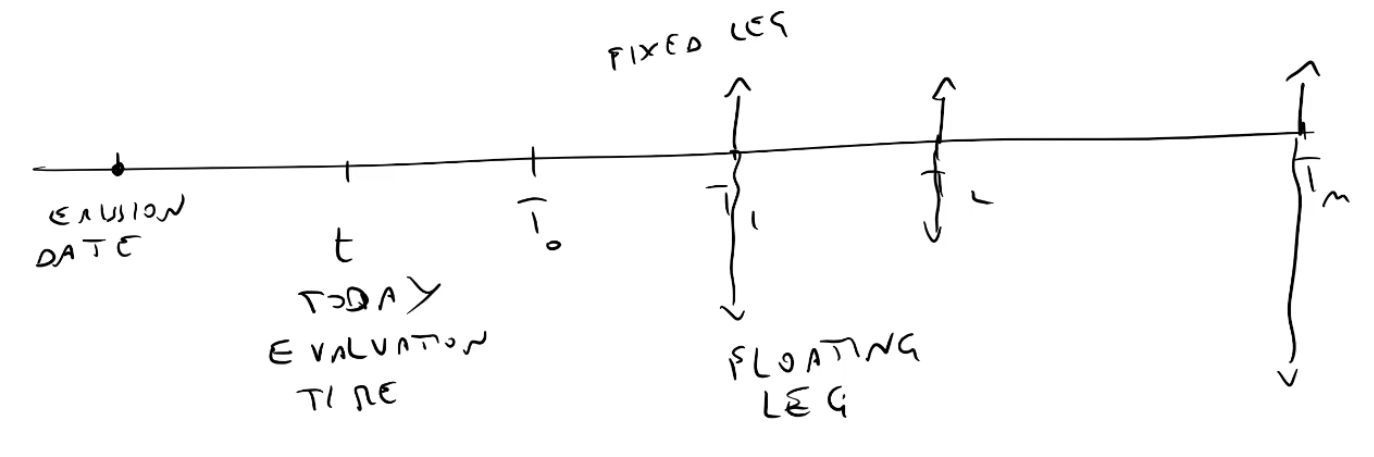
\includegraphics[scale=0.22]{fig/tmp/fig41}
    \label{fig:swap}
    \caption{Interest rate swaps}
\end{figure}
\newline There are many versions of interest rate swaps, and we will study the \emph{forward swap settled in arrears}, which is defined as follows. We denote the principal by $K$, and the swap rate by $R$. By assumption we have a number of equally spaced dates $T_0,\dots,T_n$, and payment occurs at the dates $T_1,\dots,T_n$ (not at $T_0$). If we swap a fixed rate for a floating rate (in this case the LIBOR spot rate), then, at time $T_i$, we will receive the amount
\begin{equation*}
    K\delta L(T_{i-1},T_i)
\end{equation*}
At $T_i$ we will pay the amount
\begin{equation*}
    K\delta R
\end{equation*}
so che net cash flow at $T_i$ is thus given by
\begin{equation}
    K\delta [L(T_{i-1}, T_i) - R].
\end{equation}
Basically, this is a floating bond minus a fixed bond. So, the corresponding price is given by
\begin{align*}
    price_t^{\text{SWAP}} = price_t^{\text{FLOAT}} - price_t^{\text{FIXED}}.
\end{align*}
Before the crisis this price is given by:
\begin{align}
    price_t^{\text{SWAP}} = Kp(t,T_0) - K\left(p(t,T_n) + \sum_i^n R\delta p(t,T_i)\right)
\end{align}
The swap rate $R$, which makes the whole contract fair ($price_0^{\text{SWAP}} = 0$), is different from the strike prices of the FRAs, which are fair only for the single component of the contract, and is given by
\begin{equation}
    R = \frac{p(t,T_0)-p(0,T_n)}{\delta\sum_i^n p(0,T_i)}.
\end{equation}
After the crisis, we have to adapt the formula by considering the aftermath in terms of floating and fixed bonds:
\begin{equation}
    price_t^{\text{SWAP}} = K \sum^n_{i=1}p(t,T_i) \delta (L(t,T_{i-1},T_i)-R)
\end{equation}
and the swap rate is given by a convex combination of forward LIBOR rates:
\begin{equation}
    R = \frac{\sum_{i=1}^n p(t,T_i)}{\delta\sum_{j=1}^n p(0,T_j)}L(t,T_{i-1},T_i).
\end{equation}% end part 1

\section{Non linear contracts: caps and floors} % Bjork ch. 26.8
An \emph{interest rate cap} is a financial insurance contract which protects us from having to pay more than a prespecified rate, the \emph{cap rate}, even though we have a loan at a floating rate of interest. Technically speaking, a cap is the sum of a number of basic contracts, known as \emph{caplets}, which are defined as follows:
\begin{itemize}
    \item The interval $[0,T]$ is subdivided by the equidistant points $0 = T_0,T_1,\dots,T_n = T$. We use the notation $\delta$ for the length of an elementary interval, i.e. $\delta=T_i - T_{i-1}$.
    \item The cap is working on some principal amount of money, denoted by $K$, and the cap rate is denoted by $R$.
    \item The floating rate of interest underlying the cap is not the short rate $r$, but rather some market rate, and we will assume that over the interval $[T_{i-1}, T_i]$ it is the LIBOR spot rate $L(T_{i-1}, T_i)$.
    \item Caplet $i$ is now defined as the contingent claim that has payoff at $T_i$:
    \begin{equation}\label{caplet-payoff}
        K\delta(L(T_{i-1},T_i)-R)^+
    \end{equation}
\end{itemize}
There are also \emph{floor contracts} which guarantee that the interest paid on a floating rate loan will never be below some predetermined floor rate. We now turn to the problem of pricing the caplet, and without loss of generality we may assume that $K = 1$.

\subsubsection{Before the crisis}
Before the crisis it is possible to write the LIBOR in terms of discount factor:
\begin{equation*}
    L(T_{i-1},T_i) = \frac{1-p(T_{i-1},T_i)}{\delta p(T_{i-1},T_i)}.
\end{equation*}
Substituting in eq. \eqref{caplet-payoff} (with $K=1$) we get
\begin{equation*}
    \delta(L(T_{i-1},T_i)-R)^+ = \delta\left(\frac{1-p(T_{i-1},T_i)}{\delta p(T_{i-1},T_i)}-R\right)^+
\end{equation*}
Now the idea is to collect the collect the factor $\frac{1-\delta R}{p(T_{i-1},T_i)}$ so that the payoff will correspond to a certain number of put options on the zero coupon bond:
\begin{equation}
    \frac{1-\delta R}{p(T_{i-1},T_i)}\left(\frac{1}{1+\delta R} - p(T_{i-1},T_i)\right)^+
\end{equation}
This payoff is paid at time $T_i$ but it involves quantities that are measurable with respect to the filtration at time $T_{i-1}$, $\mathcal{F}_{T_{i-1}}$. In other words, at time $T_{i-1}$ this quantity is deterministic, so in order to find the price of the caplet we only have to discount the cash flow:
\begin{equation}
    \cancel{p(T_{i-1},T_i)}\frac{1-\delta R}{\cancel{p(T_{i-1},T_i)}}\left(\frac{1}{1+\delta R}-p(T_{i-1},T_i)\right)^+ = (1+\delta R)(\text{put on } p(T_{i-1},T_i))
\end{equation}
So, in the end, the cap is a portfolio of put options on zero coupon bonds. % to continue we need a model to simulate the evolution of the discount factor, for example the B&S.

\subsubsection{After the crisis}
After the crisis we cannot consider the discount factor, so there will be a conditional expected value of the future realizations of the forward LIBOR, which in general are different for different tenors. Then, we would need a model to describe the LIBOR.

\section{Short interest rates} % bjork ch. 24
We now consider different possible specifications for the short interest rate. We altready introduced the Vašíček model, which describes the evolution of the short rate using a Brownian motion plus a drift and for which the distribution of the interest rate is gaussian. We also were able to find the price of the corresponding zero coupon bond (at least the diffusive part). Now we would like to consider other short interest rate models. \\
First, we need to extend the Feynman-Kac methodology to stochastic interest rates. If we define the infinitesimal generator
\begin{equation*}
    \mathcal{A} = \pdv{}{x}K + \frac{1}{2}\pdv[2]{}{x}H^2
\end{equation*}
we obtain the following differential equation for the evolution of the price with stochastic interest rate $r(t,x)$:
\begin{equation}
    \begin{cases}
        \pdv{F}{t} + \mathcal{A} + r(t,x)F = 0 \\
        F(T,x) = \Phi(x)
    \end{cases}
\end{equation}
The solution is given by \colorbox{cyan}{homework}
\begin{equation}
    F(t,x) = \mathbb{E}_{t,x}\left[\Phi(x_T)e^{-\int_t^T r(s,x)\,\dd s}\right]
\end{equation}
where
\begin{equation}
    \dd X = K\,\dd t + H\,\dd W
\end{equation}
Let's consider, for example, the case $r(t,x) = x$. The dynamics under the risk neutral probability measure $\Qmeas$ is
\begin{equation}
    \dd r(t) = \mu(t,r(t))\,\dd t + \sigma(t,r(t))\,\dd W^{\Qmeas}(t)
\end{equation}
In principle, we should start from the probability measure $\Pmeas$ and then try to understand which is the change of measure that leads to $\Qmeas$. However, this is a quite complicated problem because it is not clear what to impose to be a martingale, in fact the interest rate is not a traded asset. Practically, the fact that we do not know $\Pmeas$ does not matter because we want to work under $\Qmeas$, which is the probability measure that generate the prices in the market. From now on, we will consider every Brownian motion under the measure $\Qmeas$.

\subsubsection{Vašíček model}
The dynamics of the short interest rate follows the equation
\begin{equation}
    \dd r(t) = (b-ar(t))\,\dd t + \sigma\,\dd W(t), \qquad a>0
\end{equation}
This dynamics is \emph{affine}, that is the drift and the diffusion coefficients are linear combinations of the state variable (plus a constant). The short rate $r(t)$ is gaussian distributed and introducing an auxiliary process we are able to find it.

\subsubsection{Cox-Ingersoll-Ross model}
The CIR model was introduced in order to prevent the negativity of $r(t)$. It is defined by the equation
\begin{equation}
    \dd r(t) = a(b-r(t))\,\dd t + \sigma\sqrt{r(t)}\,\dd W(t)
\end{equation}
and it is an affine model (the first term and the square root of the second term are affine). A process that evolves according this equation is called \emph{squared Bessel process} and it is possible to prove that is has a strong unique solution and that if $ab>\nicefrac{\sigma}{2}$ then $\Pmeas(r(t)>0)=1$. It also holds that CIR $\sim$ Vašíček $\sim \chi^2$.

\subsubsection{Dothan model}
The dynamics is given by
\begin{equation}
    \dd r(t) = ar(t)\,\dd t + \sigma r(t)\,\dd W(t)
\end{equation}
The dynamics is not affine because the diffusive term is not the square of an affine term. The rate $r(t)$ is log-normal distributed. There are some problem in pricing the zero coupon bond because if we consider the expected value of the exponential of the integral of $r(t)$ (i.e. the zero coupon price) it can explode.

\subsubsection{Black-Derman-Toy model}
The dynamics is given by
\begin{equation}
    \dd r(t) = \theta(t)r(t)\,\dd t + \sigma(t)r(t)\,\dd W(t)
\end{equation}
where $\theta(t)$ and $\sigma(t)$ are deterministic functions that allow more flexibility to describe the process. This model is not affine.

\subsubsection{Ho-Lee model}
The dynamics is given by
\begin{equation}
    \dd r(t) = \theta(t)\,\dd t + \sigma\,\dd W(t)
\end{equation}
where $\theta(t)$ is a deterministic function and $\sigma$ is a constant. This model is the simplest specification of a more general framework -- the Heath–Jarrow–Morton framework -- which describes the dynamics of forward interest rates. The rate $r(t)$ is gaussian. There can be some stationarity issues.

\subsubsection{Hull-White model}
The dynamics is given by
\begin{equation}
    \dd r(t) = (\theta(t)-a(t)r(t))\,\dd t + \sigma(t)\,\dd W(t)
\end{equation}
The function $\theta(t)$ allows a fine calibration of the model to perfectly fit the initial yield curve.
\begin{remark}
    We will prove that $r(t)$ is affine if and only if the moment generating function is such that $\mathbb{E}[e^{r(t)}] = e^{A+Br(0)}$, where $A$ and $B$ are two deterministic functions. This has as a consequence the fact that the price of the zero coupon bond can be written in terms of $A$ and $B$:
    \begin{equation*}
        \expect_t\left[e^{-\int_t^T r(s)\,\dd s}\right] = e^{A(t,T)+r(t)B(t,T)}
    \end{equation*}
    The problem is: are we able to find the functions $A$ and $B$ for all the models above? The answer is positive, but we need to use the extension of the Feynman-Kac methodology.
\end{remark}
